%!TEX root = ../dissertation.tex

\chapter{Related Work}
\label{chapter:relatedwork}

There are several techniques that have been developed and applied to face the performance problem that we have already explained. This section will describe some of those techniques. 

This section will also present a number of systems that have goals that are similar with ours. They are good sources of ideas and points of comparison to evaluate our solution. The described systems are the most relevant ones, that take in consideration the field of architecture.

%!TEX root = ../../dissertation.tex

\section{Processing Techniques} % (fold)
\label{sec:processing_techniques}

Within the following section, a number of techniques that can be applied to improve performance of the processing and visualization of large amounts of geometry will be presented. First the \gls{LOD} in Section~\ref{sub:level_of_detail} which manages the detail that each object is generated with, and after that the \gls{OC} that manages which objects are generated.



\subsection{Level Of Detail -- JUST A COPY} % (fold)
\label{sub:level_of_detail}

Level of Detail is a technique that is used to improve the performance of the graphic pipeline. This is done by managing the complexity of the objects representation relative to some indicator.
Within this indicators, the most common one is the distance of each object to the viewer. If an object is far from the viewer a decrease on the detail will not be noticed and will save computation time. Other indicators can be the importance that is assigned for each object, relative speed or partial occlusion.

This concept is easy to understand and implement if we look at the example in the Figure~\ref{fig:LOD2}. In this figure there are five cylinders that have different detail according to the distance to the camera. In this case only the number of sides of the cylinder changes.

%\begin{figure}[htbp]
%	\centering
%	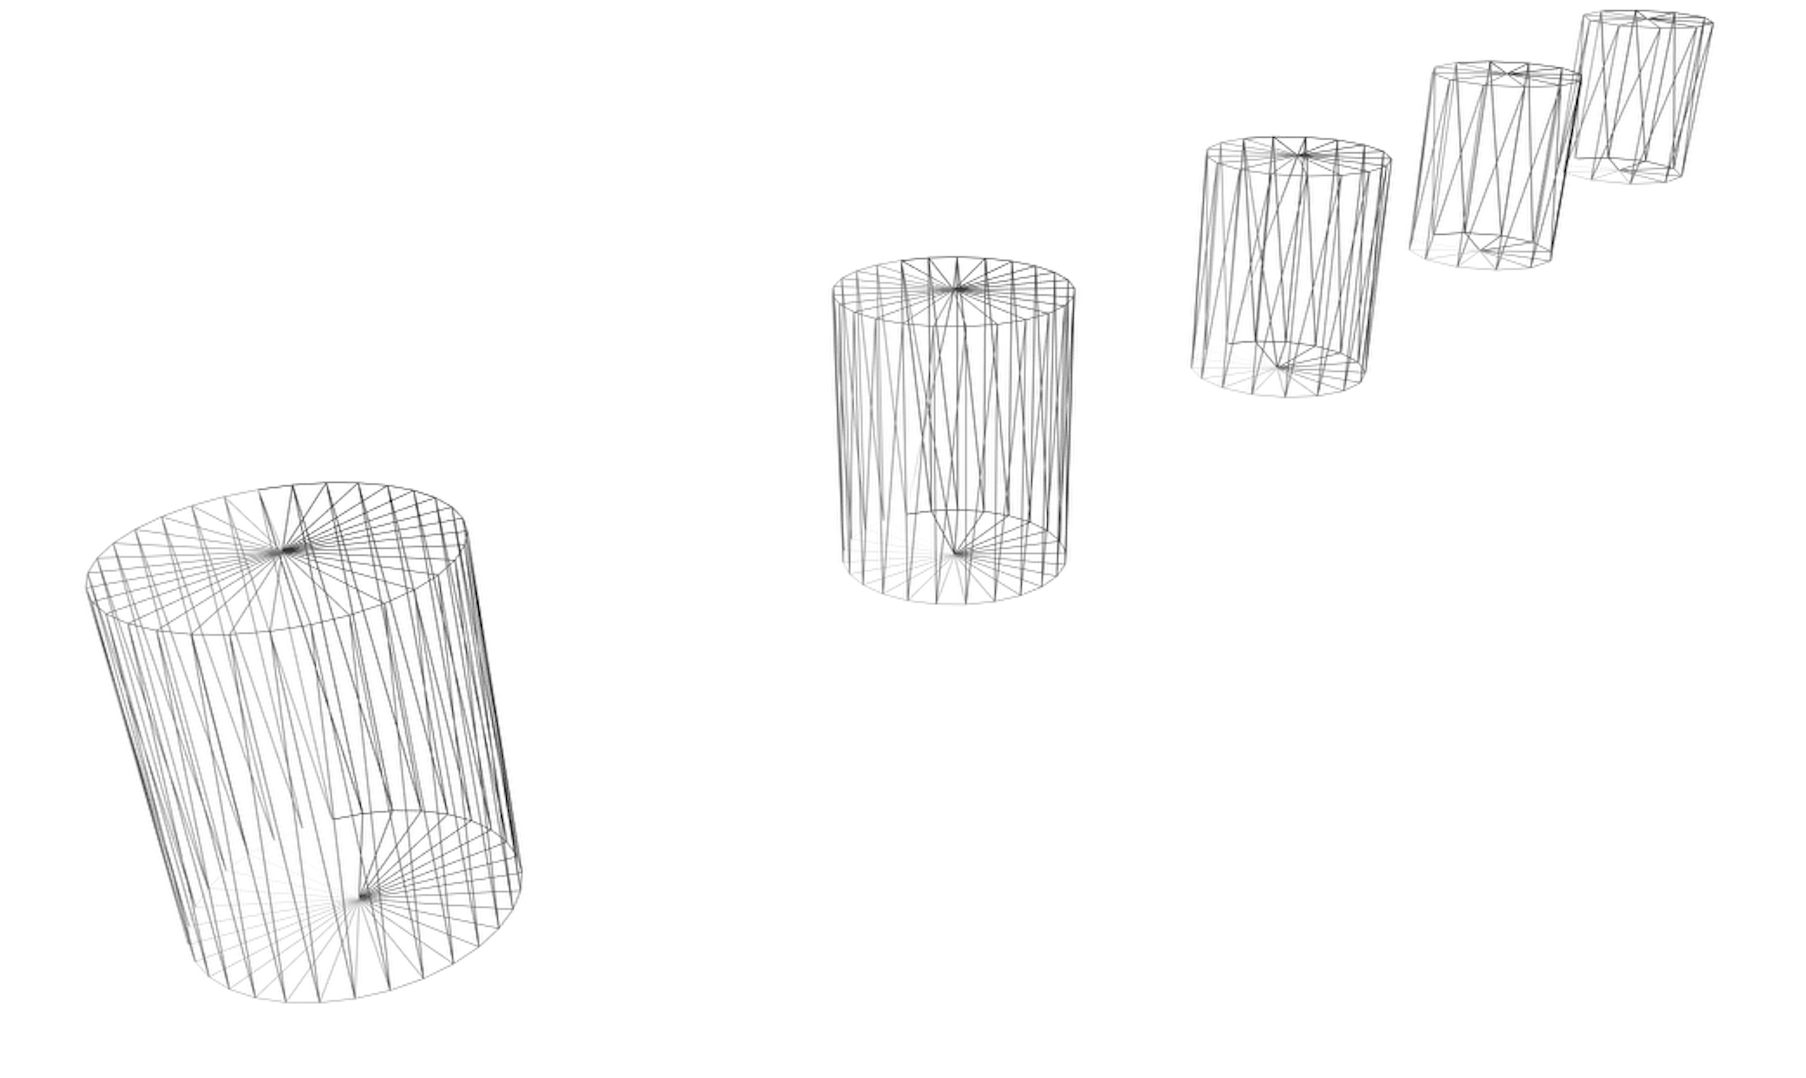
\includegraphics[width=0.95\textwidth]{imges/OpenGL/LOD3.png}
%	\caption{LOD example}
%	\label{fig:LOD2}
%\end{figure}


% subsection level_of_detail (end)

\subsection{Occlusion Culling} % (fold)
\label{sub:occlusion_culling}

Occlusion Culling is another technique that is used to improve performance. It involves determining which parts of the model are visible or not at any given moment, and with that information remove the not visible parts of the pipeline.

This technique can be implemented in different phases of the system. This can be implemented by the programmer when generating the models, only generating the parts that are visible according the the camera. But it is not easy to implement and therefore is not a good neither popular solution.

On the other end of the pipeline, it is usually done automatically by the GPU and applied to occluded faces behind other objects or out of the viewing frustum. This solution is not great because all the model is generated and, is only after that occlusion culling is applied which doesn't translate in grate performance gains.

If this concept is applied before the generation of the objects, and prevents the inclusion of large amounts of geometry through the pipeline, we can make a large improvement on performance. Figure~\ref{fig:viewingRange} is a good example. Here only the buildings that are visible from the current point are generated. This test is done prior to the generation of each object and is not hard coded within the model description.

% subsection occlusion_culling (end)

% section processing_techniques (end)

		

%!TEX root = ../../dissertation.tex


\section{Undiscovered City} % (fold)
\label{sec:undiscovered_city}

In \cite{Greuter2003} Stefan Greuter et al. presented a system that generates in real-time pseudo infinite virtual cities which can be interactively explored from a first person perspective. In their approach ``all geometrical components of the city are generated as they are encountered by the user." As shown in the Figure~\ref{fig:viewingRange} only the part of city that is inside the viewing range is generated. This method allows the visualization of massive amounts of geometry, buildings in this case, by generating in real time only the geometry that on sight, and since this subset is usually much smaller than all the geometry this results in huge benefits in performance.

\begin{figure}[htbp]
	\centering
	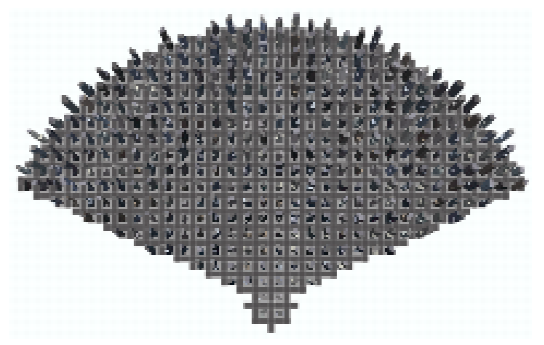
\includegraphics[width=0.85\textwidth]{images/Real-Time-procedural-generation/viewing-range.png}
	\caption{Viewing Range}
	\label{fig:viewingRange}
\end{figure}


The system uses a 2D grid that divide the terrain into square cells. The cells represent proxies for the content that will be procedurally generated. Before the content of each cell is generated, the potential visibility of it is tested, and after that, only the visible cells are filled with content.

Then the roads are created in a uniform grid pattern. This grid does not feel very natural, and with the continuation of the work, this system have become more realistic, with the join of some of the grids to create a less uniform distribution of the buildings.

The buildings within this project are generated with the simple extrusion of regular polygons. This extruded forms are composed to create complex architectural models.


(...)
% section undiscovered_city (end)
%!TEX root = ../../dissertation.tex


\section{VR Azuchi Castle} % (fold)
\label{sec:vr_azuchi_castle}


In \cite{fukuda2015}, Tomohiro Fukuda et al, presented a \gls{HD} \gls{VR} system for Historical Architectural and Urban Digital Reconstruction. They used the Azuchi Castle and the surrounding town as case study. 

They have the goal of having a real time rendering system with high accuracy and realism. With that, they face the same problems as we did. In \cite{fukuda2015}, is consider the problem of rendering large sets of objects of different scales in real time. It is also presented the various techniques they used to face this problem.

\begin{figure}[htbp]
	\centering
	\includegraphics[width=0.95\textwidth]{images/azuchi/view.png}
	\caption{Azuchi castle view}
	\label{fig:azichiview}
\end{figure}

(...)

% section vr_azuchi_castle (end)
		
%!TEX root = ../../dissertation.tex


\section{Computer Aided Tools} % (fold)
\label{sec:computer_aided_tools}
\glspl{CAD} are very powerful tools for design and architecture. Whit this tools, architects and designers are able to create, interact, and visualize their models. They support interactive manual modeling and visualization. This tools also support \gls{GD} with the implementation of \glspl{API}.


% section computer_aided_tools (end)
		
%!TEX root = ../../dissertation.tex


\section{Vizualization Library} % (fold)
\label{sec:vizualization_library}

\gls{VL}\cite{visualizationLibrary} is an OpenGL library written in C++ with focus on performance and portability. 

It is very a thin layer over OpenGL, and runs in Windows, GNU/Linux and Mac OS X operative systems. It was designed to be fine-grained platform, and is very close to the OpenGL specification. 

Since it is written in C++ which is not a very easy \gls{PL} to use, it is also not a easy platform to use.
This project was abandoned by the author in 2012, and has not received any update or maintenance since then.



% section vizualization_library (end)
		

%!TEX root = ../../dissertation.tex


\section{Rosetta} % (fold)
\label{sec:rosetta}
Rosetta \cite{lopes2011portable} is a tool for \gls{GD} that was created with very specific goals. The focus users are designers and architects, that usually do not have programming experience. So the goals was to be pedagogic, i.e. easy to learn, easy to use. To be capable to interact with the most used \gls{CAD} tools as back-ends and also implement several \glspl{PL} as front-ends.

\begin{figure}[htbp]
	\centering
	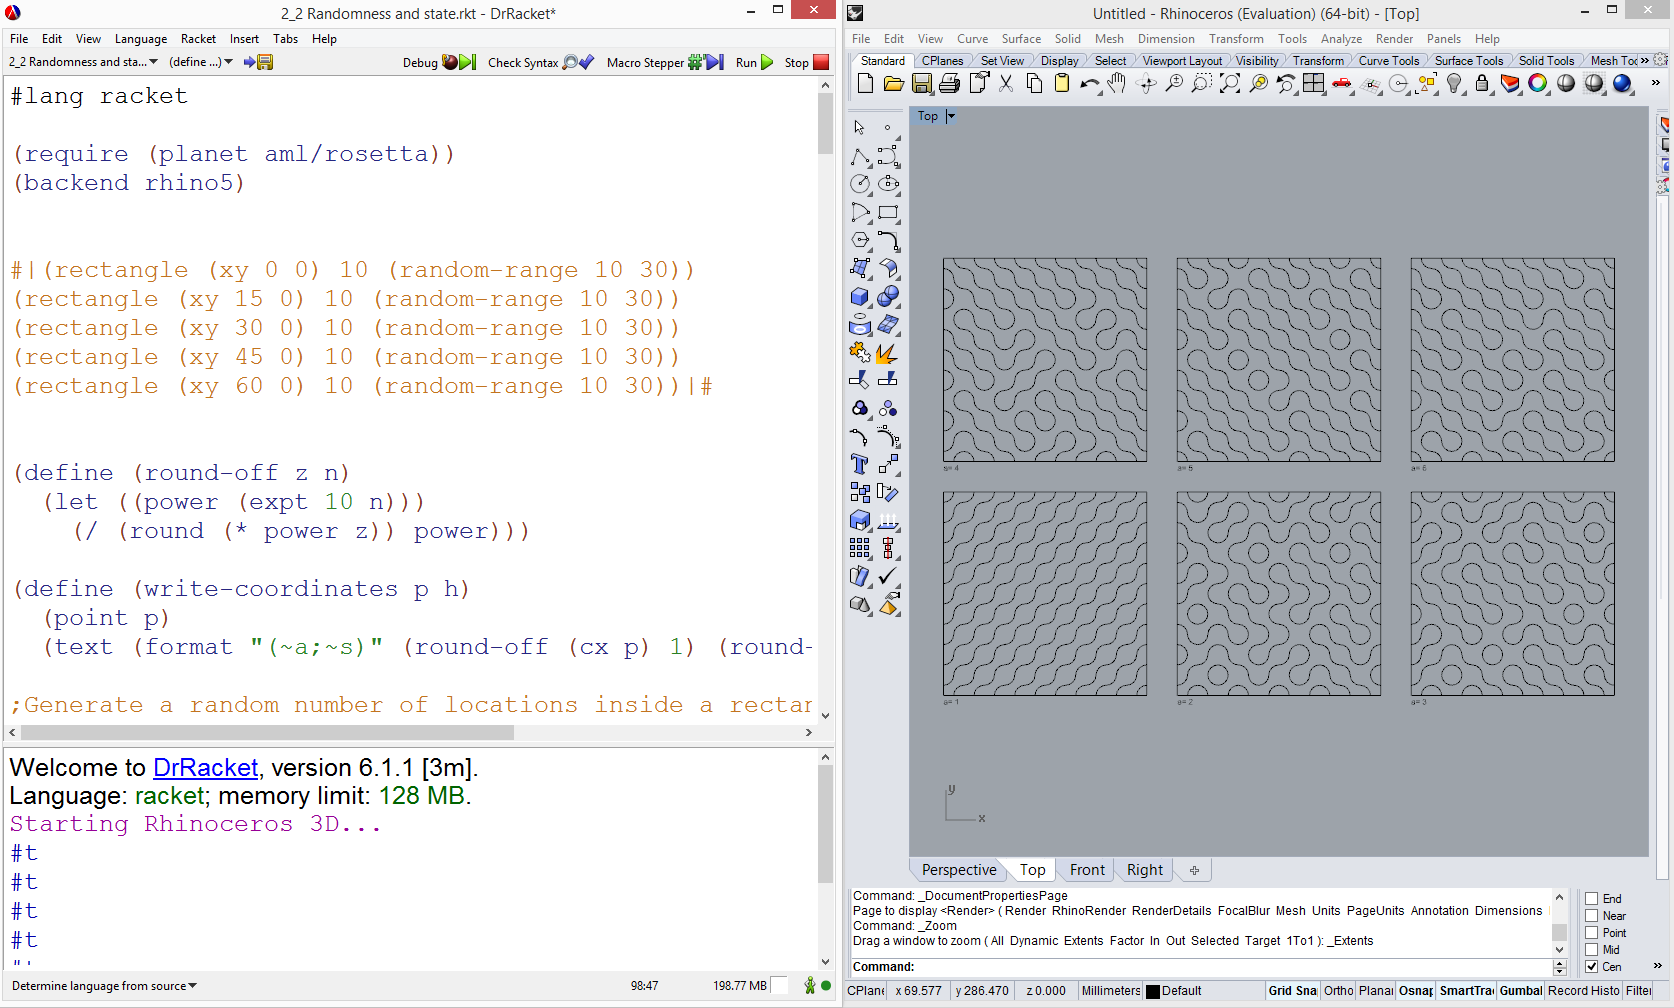
\includegraphics[width=0.95\textwidth]{images/Rosetta/Rosetta4.png}
	\caption{Rosetta IDE with Rhino}
	\label{fig:RosettaRhino}
\end{figure}

\subsection{CADs} % (fold)
\label{sub:cads}

Rosetta implements back-ends for the most used \gls{CAD} tools (Section~\ref{sub:cads}), such as AutoCad and Rhinoceros 3D. 

Since this tools where developed mainly for manual use and interaction, they have performance problems when dealing with the large amounts of geometry that tools such as Rosetta are able to generate.



% subsection cads (end)

\subsection{Visualization Library} % (fold)
\label{sub:visualization_library}

To deal with the performance problem, one extra backend was written. This backend is build using the \gls{VL} (Section~\ref{sec:vizualization_library}).

Since the \gls{VL} was created having performance as an important goal, this backend is a great improvement in what performance is concerned. It is much faster to visualize the models created within Rosetta.
This backend provides some user manual interaction, but is mostly the movement of the camera. It does not support manual modification of the model.

On the other hand, after some tests with this platform within Rosetta, the performance was not perfect yet, especially with large models. Since this project was abandoned by the author, it is not expected to have updates that would improve this issue, and also correct bugs or help with problems that are faced during the development of a tool such as Rosetta.


%Visualization

%Modeling

%Interaction

%Usability

% subsection visualization_library (end)
% section rosetta (end)

		

\section{Conclusion of related work} % (fold)
\label{sec:conclusion_of_related_work}

\begin{table}[h!]
\centering

\begin{tabular}{|l|l|l|l|l|l|}
\hline
\textbf{Tool Name}         & \textbf{Visualization Speed} & \textbf{Modeling Speed} & \textbf{Modeling} & \textbf{Interaction} & \textbf{Usability} \\ \hline
\textbf{City Engine}       & Slow                         & Fast                    & Yes               & Total                & High               \\ \hline
\textbf{\cite{fukuda2015}???} & Fast                      & -                       & None              & VR/Camera            & High               \\ \hline
\textbf{Undiscovered City} & Fast                         & -                       & None              & Camera/None?         & -                  \\ \hline
\textbf{CADs}              & Slow                         & Slow                    & Yes               & Total                & High               \\ \hline
\textbf{VL}                & Fast                         & Fast                    & Yes               & Camera               & Low                \\ \hline
\textbf{Rosetta - CADs}    & Slow                         & Fast                    & Yes               & Total                & High               \\ \hline
\textbf{Rosetta - VL}      & Fast                         & Fast                    & Yes               & Camera               & High               \\ \hline
\end{tabular}
\caption{My caption}
\label{my-label}
\end{table}


% section conclusion_of_related_work (end)
